\chapter{量子物理基础}

\section{选择题}
\exercise A

\solve 考察绝对黑体的定义。能够全部吸收各种波长的辐射能而完全不发生反射和透射的物体称为绝对黑体。故选A。

\exercise C

\solve 斯特藩-玻尔兹曼定律:$M(T)=\sigma T^4$,其中T是黑体自身温度,与环境温度无关。由于$T_A=T_B$,所以$M_A=M_B$。

\exercise C

\solve 电子绕核运动角动量的大小有表达式$L=\sqrt{l(l+1)h}$。其中$l<n$,为角量子数。%?

题给$3.464h$,即$2\sqrt{3}h$,令$\sqrt{l(l+1)h}=2\sqrt{3}h$,解得$l=3$。故选C。

\exercise A

\solve 产生光电效应的光子需满足能量大于逸出功的条件。即$h\frac{c}{\lambda}\ge eU_0$,整理得$\lambda \le\frac{hc}{eU_0}$。故选A。

\exercise D

\solve A选项,\alpha 粒子散射实验验证了原子的核式结构,与光的性质无关;B选项,辐射电磁波反应体现光的波动性;C选项,电子束的衍射图样说明了物质的波动性;D选项,光电效应反应光的粒子性,康普顿效应也能体现光的粒子性。故选D。

\exercise B

\solve 根据维恩位移定律:$\lambda_mT=b$,加热前后波长之比$\frac{\lambda_1}{\lambda_2}=\frac{6}{5}$,故$\frac{T_1}{T_2}=\frac{5}{6}$。结合斯特藩-玻尔兹曼定律:$M(T)=\sigma T^4$,所以$\frac{M_1}{M_2}=(\frac{5}{6})^4\approx\frac{1}{2}$。故选B。

\exercise C

\solve $p=\sqrt{2mE_k}=\frac{h}{\lambda}$,代入数据,得德布罗意波长$\lambda=2.0\times10^{-14}$,故选C

\exercise D

\solve 微观粒子具有的明显的波动性,以致它的某些成对物理量不可能同时具有确定的量值。$\Delta x\cdot \Delta p_x\ge h$就描述就描述了位置与动量不能同时准确确定。故选D。

\exercise C

\solve 由不确定关系,平均寿命$\Delta t\approx\frac{h}{2\pi\times2\Delta E}=\frac{6.626\times10^{-34}}{2\pi\times2\times9\times1.6\times10^{-19}}=3.5\times10^{-23}$,注意此处为约化普朗克常量,故选C。

\exercise A

\solve $h\lambda=mv,v=\frac{h}{m\lambda}\approx900\mathrm{m/s}$,故选A。

\section{填空题}

\exercise 1416

\solve $T=(\frac{M}{\sigma})^\frac{1}{4}$,解得$T=1416K$。本题注意单位统一。

\exercise 频率$\quad$绝对黑体幅射光的频率处在可见光范围内。

\solve 书中定义可知。

\exercise 半导体$\quad$绝缘体

\solve 被束缚的电子要成为自由电子或者空穴,就必须获得足够能量从价带跃迁到导带,这个能量的最小值就是禁带宽度。因此禁带宽度与导电难易程度负相关,半导体远的禁带宽度小于绝缘体。

\exercise 自发$\quad$不是$\quad$受激$\quad$是

\solve 书中定义可知。

\exercise $\sqrt{\frac{h}{2m(\nu-\nu_0)}}$

\solve $h\nu-h\nu_0=E_k=\frac{p^2}{2m}=\frac{h^2}{2m\lambda^2}$,解得$\lambda=\sqrt{\frac{h}{2m(\nu-\nu_0)}}$

\exercise 9

\solve $n=3$时;$l=0,1,2;m_l=0,\pm1,\pm2$。又由于$l<n,m_l\le l$,排列组合得$n=3$对应的电子态数目有1+3+5=9种。

\exercise 0$\quad\frac{h\nu}{c^2}$

\solve 由于光子是以光速运动,故静止质量必然为零;$E=mc^2=h\nu$,故光子的相对论质量为$\frac{h\nu}{c^2}$。

\exercise $1.45\times10^{-10}m\quad6.6\times10^{-29}m$

\solve$\lambda=\frac{h}{p}=\frac{h}{mv},\sqrt{\bar{v}^2}=\sqrt{\frac{3RT}{M}}=2735m/s$

所以$\lambda_1=\frac{6.6\times10^{-34}}{1.67\times10^{-27}}\times2735=1.45\times10^{-10}\mathrm{m}$
$\lambda_2=\frac{6.6\times10^{-34}}{1x10^{-3}}\times1\times10^{-2}=6.6\times10^{-29}\mathrm{m}$

\exercise 错误$\quad$该波函数不能满足在$x=0$连续且满足归一化条件

\solve 波函数需要连续且满足归一化条件。若该定态波函数满足连续条件,则$\psi_0=0,A=0$,故$  \int_{-\infty}^{+\infty}|\psi(x)|^2\cdot dx=0$,不满足归一化条件。故无法同时满足连续与归一化,所以是错误的。

\exercise 0.225

\solve 由势阱中粒子能级公式
\begin{gather*}
	E_n=n^2\frac{h^2}{8mL^2}\\
	E_3-E_1=h\frac{c}{\lambda}
\end{gather*}
解得$L=0.225\mathrm{nm}$。

\section{解答题}

\exercise

\solve 利用维恩位移定律以及斯忒藩-玻尔兹曼定律$T\lambda_m=b$,$M_B(T)=\sigma T^4$

太阳表面温度 
\begin{center}$T_1=\frac{B}{\lambda_{m1}}=\frac{2.898\times10^{-3}}{510\times10^{-9}}=5682\mathrm{K}$\end{center}
辐出度
\begin{center}$\qquad\qquad M_{B1}=\sigma T_1^4=5.9\times10^7\mathrm{W/m^2}$\end{center}
北极星表面温度
\begin{center}$\quad T_2=\frac{b}{\lambda_{m2}}=\frac{2.898\times10^{-3}}{350\times10^{-9}}=8280\mathrm{K}$\end{center}
辐出度
\begin{center}$\qquad\qquad M_{B2}=\sigma T_2^4=2.7\times10^7\mathrm{W/m^2}$\end{center}

\exercise

\solve (1)由$\nu=\frac{c}{\lambda}1.5\times10^{15}\mathrm{s^{-1}}$
\begin{equation}\nonumber
\begin{split}
E_k&=h\nu-W_0\\
&=6.3\mathrm{eV}-4.2\mathrm{eV}\\
&=2.0\mathrm{eV}\\
\end{split}
\end{equation}
(2)由$eU_0=E_k$,$U_0=2.0\mathrm{V}$。

(3)由$h\nu_0=W_0$
\begin{gather*}
	\nu_0=1.014\times10^{25} \mathrm{s^{-1}}
	\lambda=\frac{c}{\nu_0}=296\mathrm{nm} 
\end{gather*}

\exercise

\solve 
\[ |\psi(x)|^2=\frac{2}{a}\sin{\frac{\pi x}{a}}^2=\frac{1}{a}(1-\cos{\frac{2\pi x}{a}}) \quad (0\le x \le a) \]
$\therefore \cos{\frac{2\pi x}{a}}=-1$时,概率最大\\
即
\[ \frac{2\pi x}{a}=\pi \]
\[ x=\frac{a}{2} \]
	
\exercise

\solve 设自由电子静$m_0$,它与光子碰撞后吸收光子,然后以速度$v_2$运动,电子碰前速度为$v_1$,碰前电子和光子的夹角为$\theta_1$,碰后为$\theta_2$,如图\ref{Chp18_24}

\begin{figure}[htbp]
	\centering
	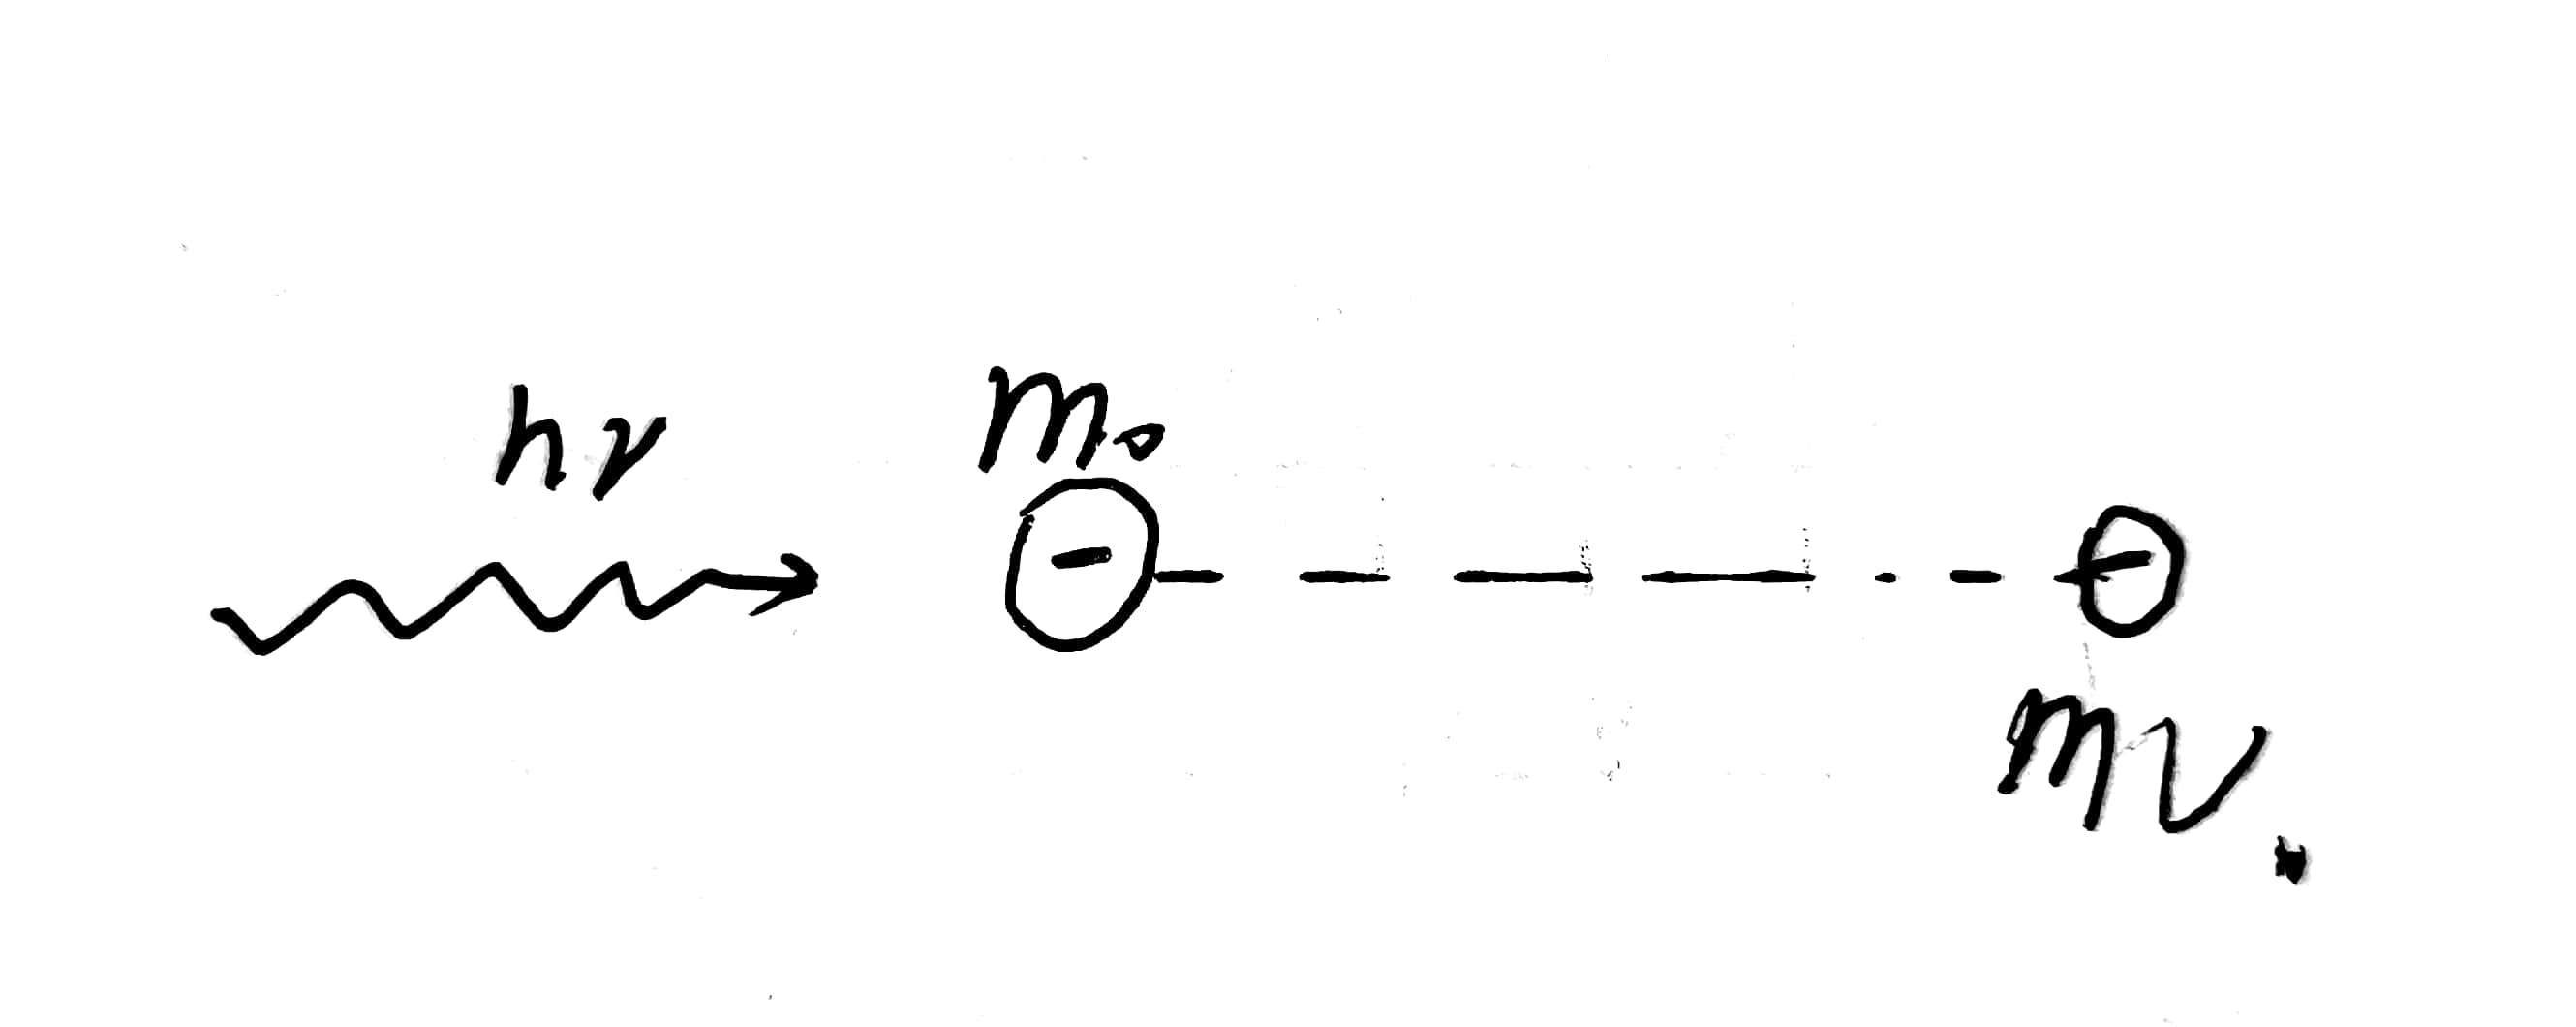
\includegraphics[width=0.6 \textwidth]{Chp18_24.jpg}
	\caption{题24图}
	\label{Chp18_24}
\end{figure}
由动量守恒
\[ x:\frac{h\nu}{c}+m_1v_1\cos\theta_1=\frac{m_0v_2}{\sqrt{1-\frac{v_2}{c}^2}}\cos\theta_2 \]
\[ y:m_1v_1\sin\theta_1=\frac{m_0v_2}{\sqrt{1-\frac{v_2}{c}^2}}\sin\theta_2 \]
解得
\[ v_2=c\sqrt{\frac{h^2\nu^2+m_1^2v_1^2c^2+2h\nu m_1v_1\cos\theta_1}{m_0^2c^4+h^2\nu^2+m_1^2v_1^2c^2+2h\nu m_1v_1\cos\theta_1}} \]

若能量全部转移,由能量守恒
\[ h\nu+m_1c^2=\frac{m_0}{\sqrt{1-\frac{v_2'}{c}^2}}\cdot c^2 \]
解得
\[v_2'=\frac{c\sqrt{h^2\nu^2+(m_1^2-m_0^2)c^4+2h\nu m_1c^2}}{h\nu+m_1c^2}  \]
由于$v_2\neq v_2'$,说明光子不可能把能量全部转移给电子。